%!TEX root = ../main.tex

\chapter{Background}
\label{chp:background}

\section{The Web of Data}
\label{sec:web-of-data}

%% Semantic Web
The World Wide Web was originally designed to be a space where documents are connected by links without semantic value, and most of these documents are designed for humans to read, not for machines to process. For this reason, Tim Berners-Lee in 2001 introduced the idea of the Semantic Web. In particular, the Semantic Web is an enhancement of the current Web that aims to create a web of data, in which information has a well-defined meaning and can be easily read and processed by programs \cite{berners2001semantic}.

Due to this machine-comprehensible capacity, the Semantic Web has enormous potential to automate daily tasks in our lives and is helping to advance scientific and health care fields \cite{feigenbaum2007semantic}, such as drug discovery and clinical research, but also in the automotive industry, in the enhancement of cultural heritage, etc\dots.\footnote{\url{https://www.w3.org/2001/sw/sweo/public/UseCases/}} In this context, ontologies play a fundamental role in supporting interoperability and common understanding between different web applications and services, solving the problem of semantic heterogeneity \cite{taye2010understanding}.

%% Ontology
\paragraph*{}
Although there are different definitions of "ontology" \cite{taye2010understanding}, in computer science, an ontology is defined as an "explicit and formal specification of a shared conceptualization" \cite{gruber1995toward}, where conceptualization means a simplified view of the world we wish to represent. An ontology is made up of four main types of components, which are (1) \textit{classes} (or \textit{concepts}), which describe concepts in the domain; (2) \textit{instances} of classes, which represent specific objects or elements of a class; (3) \textit{properties} (or \textit{slots}), which are used to express relationships between a first concept in the domain and a second concept in the range; (4) \textit{axioms} (or \textit{role restrictions}), which are used to impose constraints on the values of instances and classes \cite{taye2010understanding, noy2001ontology}. In addition to the interoperability problem, ontologies are also used to satisfy the following needs:

\begin{itemize}
    \item To share common understanding of the structure of information among people or software agents;
    \item To enable reuse of domain knowledge;
    \item To make domain assumptions explicit;
    \item To separate domain knowledge from the operational knowledge
    \item To analyze domain knowledge \cite{noy2001ontology}.
\end{itemize}

Along with ontologies, controlled vocabularies, taxonomies, and thesauri are other resources used in different domains, in particular the medical one \cite{ivanovic2014overview}. A controlled vocabulary is a closed list of named subjects, called \textit{terms}, which is usually used for classification. A taxonomy is a subject-based classification that organizes terms in a controlled vocabulary into a hierarchy. Finally, a thesaurus extends taxonomies, allowing making other statements about the subjects and providing a much richer vocabulary \cite{ivanovic2014overview}.

%% Linked Data and Web of Data
\paragraph*{}
In 2006, Tim Berners-Lee used for the first time the term Linked Data to describe the structured and interlinked data that populate the Semantic Web \cite{berners2006linked}. He also introduced a set of rules, also known as the Linked Data Principles, to provide some best practices for publishing and connecting data on the Web \cite{bizer2011linked}. These principles, published by \ac{W3C}, are the following:

\begin{enumerate}
    \item Use \acsp{URI} as names for things;
    \item Use \acs{HTTP} \acsp{URI} so that people can look up those names;
    \item When someone looks up \acsp{URI}, provide useful information, using standards such as \acs{RDF} and \acs{SPARQL};
    \item Include links to other \acsp{URI} so that they can discover more things.
\end{enumerate}

The two main fundamental technologies for Linked Data are \acp{URI} and \ac{HTTP}. In particular, \acp{URI} are used to identify any entity that exists in the world, while \ac{HTTP} provides a simple and universal mechanism for retrieving the resources to which they refer. These two technologies are integrated in \ac{RDF}, which provides a graph-based data model to structure and link data that describe entities in the world \cite{bizer2011linked}. Using \acp{HTTP}, \acp{URI}, and \ac{RDF}, Linked Data builds on the architecture of the Web, called the Web of Data. This means that the Web of Data shares many properties with the traditional Web, which are:

\begin{itemize}
    \item Web of Data can contain any type of data;
    \item Anyone can publish data on the Web of Data;
    \item Publishers are not restricted in the choice of vocabularies used to represent the data;
    \item Entities are connected by \ac{RDF} links \cite{bizer2011linked}.
\end{itemize}

However, in addition to those of the traditional Web, the Web of Data also has the following characteristics:

\begin{itemize}
    \item Data are separated from formatting and presentational aspects;
    \item Data is self-describing;
    \item Data access is simplified by the use of the \ac{HTTP} and \ac{RDF} standards;
    \item Web of Data is open, and new data sources can be discovered at run-time by following \ac{RDF} links \cite{bizer2011linked}.
\end{itemize}

%% Technology stack
\paragraph*{}
Semantic Web and Linked Data are empowered by technologies developed by the \acl{W3C} such as \acs{RDF}, \acs{OWL}, serialization formats (Section \ref{sec:rdf-owl-formats}), and \acs{SPARQL} (Section \ref{sec:sparql}).\footnote{\url{https://www.w3.org/2001/sw/wiki/Main_Page}}

%% Linked Open Data and Five Stars
\section{The five stars of Open Data}
\label{sec:opendatastars}

%% custom command for stars
\definecolor{StarColor}{HTML}{FECD70}
\newcommand{\Stars}[1]{\clone{#1}{\textcolor{StarColor}{\Large$\bigstar$}}}

Linked Data does not have to be open and can be used internally, such as for personal data. When Linked Data is released under an open license that does not impede its reuse for free, such as Creative Commons CC-BY\footnote{\url{https://creativecommons.org/}} or the Italian Open Data License\footnote{\url{https://www.dati.gov.it/content/italian-open-data-license-v20}}, we can use the term \ac{LOD} \cite{berners2006linked}. In 2010 Tim Berners-Lee developed a star rating system to define and classify Linked Open Data, "in order to encourage people, especially government data owners, along the road to good linked data" \cite{berners2006linked}. The star rating system assigns a star if the information is publicly available under an open license, even if the information is a photo or an image scan of a table. The more stars the information gets, the easier it will be for people (and machines) to use it \cite{berners2006linked}.

\begin{enumerate}[%
align=right,
leftmargin=*,
labelindent=\widthof{\Stars{5}}
]
    \item[\Stars{1}] Available on the Web (any format) but with an open license to be Open Data
    \item[\Stars{2}] Available as machine-readable structured data (e.g., Excel instead of an image scan of a table)
    \item[\Stars{3}] Available in a non-proprietary format (e.g., \acs{CSV} instead of Excel)
    \item[\Stars{4}] Use \acp{URI} to identify things, so that people can point at your stuff
    \item[\Stars{5}] Data are linked to other people's data to provide context
\end{enumerate}

However, as the information receives a greater number of stars, both the benefits for consumers and the costs for the publisher increase. In particular, a five-stars data let consumers discover new data of interest, access to the data schema, reuse parts of the data, and link it to other places. They also do not have to pay for tools in order to read the data (e.g., Excel), and they can download and export the data into other formats and process them. On the other hand, to make these data available, publishers must invest time and resources in slicing and organizing the data, assigning \acp{URI} to the data items, thinking about how to represent them, linking the data with other data on the Web and making them discoverable \cite{bauer2011linked}.

%% RDF, OWL and Serialization Formats
\section{RDF, OWL, and serialization formats}
\label{sec:rdf-owl-formats}

%% RDF
The \acf{RDF} is a \ac{W3C} graph-based standard model to represent information about resources on the Web (including documents, people, physical objects, and abstract concepts). Using \ac{RDF}, machines can process information on the Web using common parsers and processing tools, and information can be exchanged between different applications without losing meaning \cite{world2014rdfprimer}. In particular, in recent years \ac{RDF} has become the \textit{de-facto} standard for publishing Linked Data on the Web. The core structure of the \ac{RDF} syntax is a set of statements, called \textit{triples}, because they consist of three elements: a \textit{subject}, a \textit{predicate}, and an \textit{object}, following the structure \verb#<subject> <predicate> <object>#, which can be visually represented in Figure \ref{fig:rdf-graph-structure} \cite{world2014rdfconcepts}.

\begin{figure}[!ht]
    \centering
    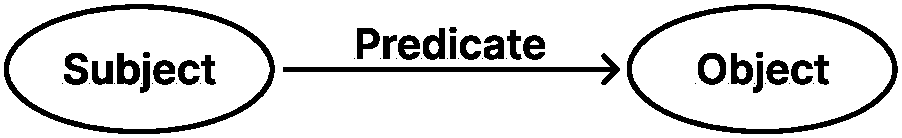
\includegraphics[width=0.55\columnwidth]{images/rdf-graph-structure.pdf}
    \caption{The structure of a triple, with two nodes and a predicate connecting them.}
    \label{fig:rdf-graph-structure}
\end{figure}

The subject and the object represent the two resources being related. The relationship that goes from the subject to the object is called \textit{property}, and its nature is represented by the predicate. A set of statements generate a direct graph, called RDF graph, where subjects and objects are the nodes of the graph, and the predicates form the arcs. For example, the set of triples below produces the graph shown in Figure \ref{fig:rdf-graph-examle} \cite{world2014rdfprimer}.

\begin{verbatim}
<Bob> <is a> <person>.
<Bob> <is a friend of> <Alice>.
<Bob> <is born on> <the 4th of July 1990>.
<Bob> <is interested in> <the Mona Lisa>.
<the Mona Lisa> <was created by> <Leonardo da Vinci>.
<the video 'La Joconde à Washington'> <is about> <the Mona Lisa>
\end{verbatim}

\begin{figure}[!ht]
    \centering
    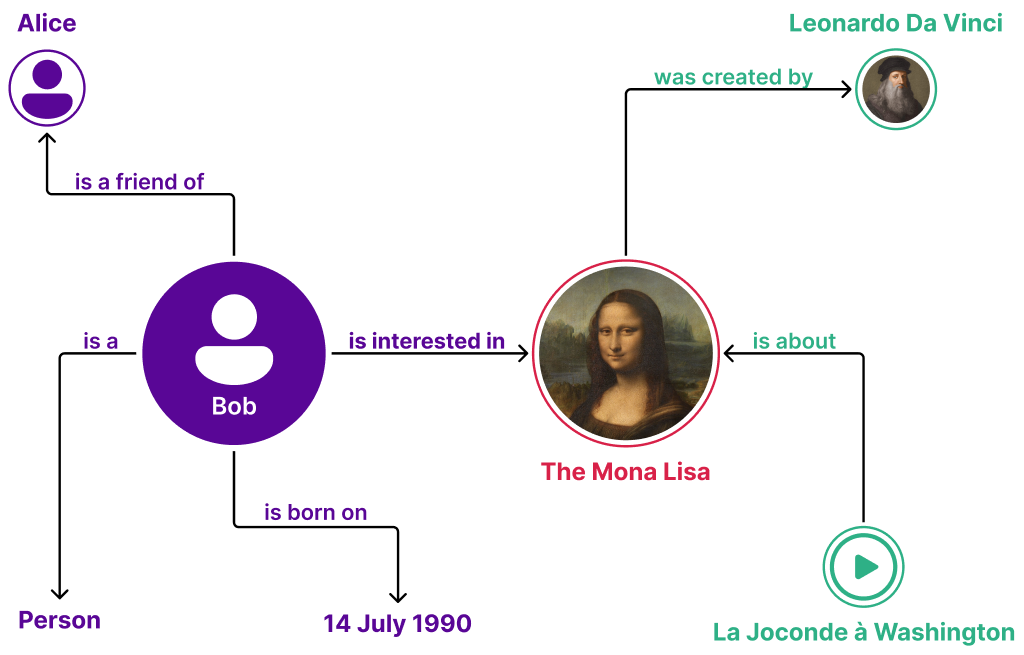
\includegraphics[width=0.95\columnwidth]{images/rdf-graph-example.pdf}
    \caption{The example of the \ac{RDF} graph presented by \ac{W3C}.}
    \label{fig:rdf-graph-examle}
\end{figure}

In an \ac{RDF} graph, resources may be represented using an \ac{IRI}, a \textit{literal value} or a \textit{blank node}. An \ac{IRI} is a generalization of \ac{URI}, where non-\acs{ASCII} characters are allowed in the \ac{IRI} character string. \acp{IRI} identify resources, and can appear in all three positions of a triple. In the example above, the \ac{IRI} for Leonardo Da Vinci in DBpedia\footnote{\url{https://www.dbpedia.org/}} is \url{http://dbpedia.org/resource/Leonardo_da_Vinci}.

Literals are basic values such as strings, dates, and numbers. In the \ac{RDF} graph literals can only be used as objects, and consists of two or three elements, which are: (1) the value itself; (2) an \ac{IRI} that identifies the \textit{datatype} (string, number, date, etc.); (3) if and only if the datatype is a \texttt{rdf:langString},\footnote{\url{http://www.w3.org/1999/02/22-rdf-syntax-ns\#langString}} a \textit{language tag} (such as \texttt{en}, \texttt{it}, \texttt{fr}, etc.) \cite{world2014rdfconcepts}.

Finally, blank nodes can appear in the subject and object position of a triple and are used to represent resources without using a \ac{IRI} \cite{world2014rdfprimer}.

%% OWL
\paragraph*{}
In Section \ref{sec:web-of-data} ontologies and vocabularies are presented as a core element for creating the Semantic Web. The \ac{RDF} data model does not provide semantic information about the resources. For this reason, \ac{RDF} provides the \ac{RDFS} language, that allows to define semantic characteristics of data. \acl{RDFS} uses the notion of \textit{class} to classify resources, while uses the \textit{type} property to define a relation between an instance and its class. \acl{RDFS} also allows defining type restrictions on subject and objects of particular triples through \textit{domain} and \textit{range} restrictions. Finally, with \acl{RDFS} it is also possible to define hierarchies of classes and properties, using \textit{subClassOf} and \textit{subPropertyOf} predicates \cite{world2014rdfprimer}. All of these modeling constructs provided by \acl{RDFS} are summarized in Table \ref{tab:rdfs-constructs}.

\begin{table}[!ht]
    \centering
    \doublespacing
    \begin{tabular}{|l|l|l|}
        \hline
        \multicolumn{1}{|c|}{\textbf{Construct}} & \multicolumn{1}{c|}{\textbf{Syntactic form}} & \multicolumn{1}{c|}{\textbf{Description}}            \\ \hline
        \textbf{Class}                           & C rdf:type rdfs:Class                        & C is an RDF class                       \\ \hline
        \textbf{Property}                        & P rdf:type rdf:Property                      & P is an RDF property                    \\ \hline
        \textbf{type}                            & I rdf:type C                                 & I is an instance of C         \\ \hline
        \textbf{subClassOf}                      & C1 rdfs:subClassOf C2                        & C1 is a subclass of C2           \\ \hline
        \textbf{subPropertyOf}                   & P1 rdfs:subPropertyOf P2                     & P1 is a sub-property of P2 \\ \hline
        \textbf{domain}                          & P rdfs:domain C                              & domain of P is C             \\ \hline
        \textbf{range}                           & P rdfs:range C                               & range of P is C              \\ \hline
    \end{tabular}
    \caption{The main modeling constructs provided by RDF Schema.}
    \label{tab:rdfs-constructs}
\end{table}

However, in 2004 the \acl{W3C} presented \ac{OWL}, a more complete language for publishing and sharing ontologies on the Web \cite{bechhofer2004owl}, and replaced in 2009 and then in 2012 by \ac{OWL} 2. \ac{OWL} 2 is a Semantic Web language to represent rich and complex knowledge about things, groups of things, and relations between things. In addition, since \ac{OWL} is a computational logic-based language, the knowledge expressed in \ac{OWL} can be reasoned with by computer programs either to verify the consistency of that knowledge or to make implicit knowledge explicit. A \ac{OWL} document, called \textit{ontology}, can be published in the World Wide Web and may refer to or be referred from other \ac{OWL} ontologies \cite{hitzler2009owl}. In \ac{OWL} 2 knowledge is represented by statements, called \textit{axioms}. Axioms normally refer to objects of the world and describe them by putting them into categories or saying something about their relation. In \ac{OWL} 2 objects, categories and relations are called \textit{entities}, and in particular objects are denoted as \textit{individuals}, categories as \textit{classes} and relations as \textit{properties}. Moreover, properties are further subdivided into (1) \textit{object properties} that relate objects to objects; (2) \textit{datatype properties} that assign data values to objects; (3) \textit{annotation properties} that encode information about the ontology itself. Finally, names of entities can be combined into \textit{expressions} using \textit{constructors} to form complex descriptions from basic ones \cite{hitzler2009owl}.

\paragraph*{}
In order to publish \ac{RDF} data on the Web, the \ac{RDF} graphs need to be serialized. Today there are several serialization formats, but the most famous one are: N-Triples, Turtle, RDF/XML, and JSON-LD. These formats are briefly described below, reporting as example of small excerpt of DBpedia\footnote{\url{https://www.dbpedia.org/}} is reported.

\paragraph*{N-Triples\footnote{\url{https://www.w3.org/TR/n-triples/}}} It's one of the simplest formats, formed by sequences of \ac{RDF} triples. Each statement is formed by the subject, predicate, object, and a ".", that are separated by white space.

\begin{verbatim}
<https://dbpedia.org/page/Jotaro_Kujo>
  <https://dbpedia.org/ontology/relative>
    <https://dbpedia.org/page/Joseph_Joestar> .
\end{verbatim}

\paragraph*{Turtle\footnote{\url{https://www.w3.org/TR/turtle/}}} It's a common data format for serializing \ac{RDF} graphs that introduces some features to N-Triples language. In particular, it introduces the use of \texttt{@base} \ac{IRI} and relative \acp{IRI}, \texttt{@prefix} and prefixed names, predicate lists separated by ";", object lists separated by ",", and the representation of \texttt{rdfs:type} with the token \texttt{a}.

\begin{verbatim}
@prefix dbr: <https://dbpedia.org/page/> .
@prefix dbo: <https://dbpedia.org/ontology/> .

dbr:Jotaro_Kujo dbo:relative dbr:Joseph_Joestar .
\end{verbatim}

\paragraph*{RDF/XML\footnote{\url{https://www.w3.org/TR/rdf-syntax-grammar/}}} Expresses \ac{RDF} graphs as an \acs{XML} document. The nodes and predicates are represented in \acs{XML} terms: element names, attribute names, element contents and attribute values.

\begin{verbatim}
<rdf:RDF xmlns:db="https://dbpedia.org/page/"
  xmlns:dbo="https://dbpedia.org/ontology/"
  xmlns:rdf="http://www.w3.org/1999/02/22-rdf-syntax-ns#"
  xml:base="http://www.ldf.fi/service/rdf-serializer/">
  <rdf:Description
    rdf:about="https://dbpedia.org/page/Jotaro_Kujo">
    <dbo:relative
      rdf:resource="https://dbpedia.org/page/Joseph_Joestar"/>
  </rdf:Description>
</rdf:RDF>    
\end{verbatim}

\paragraph*{JSON-LD\footnote{\url{https://www.w3.org/TR/json-ld/}}} Serializes \ac{RDF} graphs into \ac{JSON}. The syntax is designed to easily integrate into deployed systems that already use \ac{JSON}. It's intended to be a way to use Lined Data in Web-based programming environments, to build interoperable Web services, and to store Linked Data in \ac{JSON}-based storage engines.

\begin{verbatim}
[
  {
    "@id": "https://dbpedia.org/page/Joseph_Joestar"
  },
  {
    "@id": "https://dbpedia.org/page/Jotaro_Kujo",
    "https://dbpedia.org/ontology/relative": [
      {
        "@id": "https://dbpedia.org/page/Joseph_Joestar"
      }
    ]
  }
]
\end{verbatim}

%% SPARQL
\section{SPARQL}
\label{sec:sparql}

%% protegè

%% virtuoso

%% ontopia

%% svelte